\documentclass{applemlr}

\usepackage{amsmath, amssymb}
\usepackage{graphicx}
\usepackage{booktabs}
\usepackage{tabularx}
\usepackage{array}
\usepackage{enumitem}
\usepackage{listings}
\usepackage{caption}
\usepackage{float}

\setcounter{tocdepth}{2}
\setlist[itemize]{leftmargin=*, itemsep=0.4em}
\setlist[enumerate]{leftmargin=*, itemsep=0.4em}
\newcolumntype{Y}{>{\centering\arraybackslash}X}

\definecolor{listingbg}{gray}{0.95}
\definecolor{listingborder}{HTML}{D0D3D4}
\definecolor{listingcomment}{HTML}{5E8050}
\definecolor{listingkeyword}{HTML}{007AFF}

\lstdefinestyle{aiproject}{
  backgroundcolor=\color{listingbg},
  frame=single,
  framerule=0.4pt,
  rulecolor=\color{listingborder},
  basicstyle=\ttfamily\footnotesize,
  keywordstyle=\color{listingkeyword}\bfseries,
  commentstyle=\color{listingcomment},
  numbers=left,
  numberstyle=\scriptsize\color{listingkeyword},
  stepnumber=1,
  numbersep=6pt,
  breaklines=true,
  columns=fullflexible,
  captionpos=b,
  keepspaces=true
}


\usepackage{xcolor}       % 用于颜色定义
\usepackage[most]{tcolorbox} % 引入 tcolorbox 宏包

\newtcbox{\code}{
  on line,
  nobeforeafter, % 确保它是一个行内命令
  colback=black!10, % 背景颜色 (10%的黑色，即浅灰色)
  colframe=black!60, % 边框颜色 (60%的黑色)
  boxrule=0.5pt,    % 边框粗细
  arc=2pt,          % 圆角大小
  boxsep=0pt,       % 内部文字与边框的间距
  left=3pt, right=3pt, top=1pt, bottom=1pt, % 分别设置四个方向的间距
  tcbox raise base,
  fontupper=\ttfamily % 盒子内的文字使用打字机字体
}




\title{基于Qwen大模型的AI智能衣柜穿搭助手}

\author{武昂达}
\author{刘景鲁豫}
\author{姚文熙}
\affiliation{上海交通大学自动化与感知学院}

\metadata[课程信息]{人工智能算法实践}
\metadata[提交日期]{2026 年 6 月 x 日}

\abstract{
待报告全部完成后补充
}

\begin{document}

\maketitle

\tableofcontents
\newpage

\section{引言}

对于现在的大学生而言，日常生活中有许多看似轻松不要紧，实际研究起来却耗费时间和精力的事情，穿搭就是其中的一个典型例子。
每天上课、实验、社团、面试或出游等等，不同场合下的衣着风格有不同要求；
但现实中，许多同学往往因为时间紧、经验不足，或是懒得反复搭配，最后长期停留在几套固定组合上。
例如许多男同学夏天习惯上身短袖加条黑短裤，冬天则是羽绒服加条长裤，不用太过考虑，一套就能管一周。
这样的选择虽然足够方便，但却很难体现个人风格，无形中让生活少了一些精致，还容易让衣柜中已有的衣物利用率变低。
而随着大语言模型与多模态生成技术的发展，AI 工具展现出的能力已经逐渐从单纯回答问题“进化”为共同参与决策。
因此，我们想到搭建一个 AI 衣柜助手，让它来帮助我们参谋每天应该穿些什么。

我们认为穿搭推荐并不只是一个简单的文本生成问题，
直接向大模型询问“今天穿什么”虽然能够得到一些建议，但这类建议往往比较泛泛，甚至会推荐用户根本没有的衣服。
一个真正可用、可靠的 AI 智能衣柜助手，需要同时理解用户的基本信息、场合需求、风格偏好、已有衣物以及历史反馈，并在这些约束下给出具体、可执行的搭配方案。
因此，我们希望将大语言模型从一次性的聊天工具，进一步构建成一个\textbf{面向日常穿搭决策的个性化 AI Agent。}

基于这个目标，我们\textbf{设计并实现了 AIWardrobe  ————\ 一个基于 Qwen 大模型的 AI 智能衣柜穿搭助手。}
这个助手支持用户创建个人档案，维护自己的衣柜，并通过自然语言输入当天的场景、心情、天气或风格需求。
为了避免推荐结果脱离现实，助手在生成穿搭方案前会结合用户衣柜信息，并利用人工收集和描述的 150 余条穿搭案例构建参考案例库，通过语义向量检索找到与当前需求相近的搭配风格。
与此同时，系统还会从用户对话中抽取长期偏好，例如喜欢的颜色、版型、风格以及明确不喜欢的元素，使后续推荐能够逐渐贴近用户个人习惯。

从技术实现上来看，我们的项目搭建了“需求解析—安全审核—案例检索—衣柜约束—方案生成—可视化展示—偏好更新”的完整链路。
前端负责用户信息录入、衣柜编辑、对话交互和结果展示，后端负责模型调用、RAG 检索、Prompt 组织、数据存储与异常兜底。
穿搭助手不仅生成三套文字化穿搭建议，还提供参考案例证据和虚拟上身效果，使用户能够更直观地判断推荐是否符合自己的需求。
因此，相较于单纯的大模型问答，\textbf{我们的穿搭助手更强调穿搭的系统性、个性化和可落地性。}

我们的报告将围绕 AIWardrobe 助手的设计与实现展开说明。
首先，我们将介绍相关工作与项目使用的数据来源；
之后，我们会阐述系统架构、RAG 检索机制、用户偏好记忆、衣柜约束与多模态生成流程等链路流程涉及到的结构与技术；
最后通过具体实验分析助手在穿搭推荐、个性化适配和安全可靠性方面的表现，并对我们的项目进行进一步发展的展望。


\section{相关工作}

本项目涉及的相关工作主要可以从四个方面展开：
个性化穿搭推荐、检索增强生成、大语言模型智能体与个性化记忆、多模态图像生成与虚拟上身。
这些方向分别对应项目中的推荐方案、参考案例检索、用户偏好记忆和上身可视化模块。

\subsection{个性化穿搭推荐}

穿搭推荐不同于普通商品推荐，它不仅要判断用户是否喜欢某件单品，还要考虑多件衣物之间的组合关系。
Han et al. 提出利用序列模型学习服装单品之间的兼容性，将一套 outfit 看作多个 fashion item 组成的序列，
从而判断整体搭配是否合理 \citep{han2017learning}。
后续也有工作使用 Transformer 建模 outfit 中不同单品的关系，
例如 Sarkar et al. 的 OutfitTransformer 就用于学习整套穿搭的表示，
从而支持后续服装兼容性判断和推荐任务 \citep{sarkar2023outfittransformer}。
这些研究说明，穿搭推荐的重点并不是简单推荐单件衣服，而是理解颜色、版型、风格、材质和场景之间的组合关系。

不过，现实中的穿搭推荐还需要考虑“可穿性”。如果系统推荐了用户衣柜中不存在的衣服，即使风格上合理，也难以真正落地。
因此，我们的项目在生成穿搭方案时加入了用户衣柜约束，使模型的推荐结果尽量围绕用户已有衣物展开。
这也是本项目区别于普通聊天式穿搭模型的重要特点。

\subsection{检索增强生成 (RAG)}

检索增强生成是一类将外部知识检索与大模型生成相结合的方法。
Lewis et al. 提出的 RAG 框架将参数化生成模型与非参数化知识索引结合，
在生成答案前先检索相关文档，再基于检索结果进行回答 \citep{lewis2020retrieval}。
这一思想能够在一定程度上减少模型幻觉，同时提升生成结果与具体任务之间的相关性。
我们意识到用户的衣柜与模型返回的穿搭结果也应该具有这种强相关性，因而这启发我们在项目中运用 RAG 技术让大模型生成穿搭。

在我们的项目中，RAG 并不是用于检索百科知识，而是用于检索穿搭参考案例。
在调用模型前，我们人工整理了 150 余条社交媒体穿搭案例，并为每条案例标注了风格、颜色、场景和搭配简介。
当用户输入穿搭需求后，系统会根据语义向量检索相似案例，并将这些案例作为大模型生成穿搭方案的参考。
通过这种方法，可以让模型的推荐结果更具体、更“有人味”，也更接近真实穿搭场景。

\subsection{大语言模型智能体与个性化记忆}

近年来，大语言模型逐渐从单轮问答工具发展为能够调用工具、保存记忆并执行多步骤任务的智能系统。
Park et al. 提出的 Generative Agents 展示了如何为语言模型代理构建记忆、反思和规划机制，
使其能够在虚拟环境中表现出连续的行为 \citep{park2023generative}。
这一思路启发我们将穿搭助手设计为一个具有状态和记忆的个性化 Agent，而不是一次性的文本生成器。

对于我们的项目而言，用户的历史偏好非常重要。
若用户曾表达“不喜欢高跟鞋”“喜欢宽松版型”或“偏好冷色系”等个性化偏好，那么这些信息都应该影响后续推荐。
因此，助手应当主动从对话中抽取 likes、dislikes 和 contextual preferences 等结构化偏好，并在后续生成中作为约束使用。
同时，为了避免用户输入中含有越权请求或有 prompt injection 等影响模型的行为，我们也在需求解析阶段加入了安全审核。

\subsection{多模态生成与虚拟上身}

穿搭推荐天然具有视觉属性。单纯的文字建议虽然能够说明“上衣搭配什么裤子”，但用户往往仍然需要在脑中想象整体效果。
这就会为用户带来额外的思考成本，尤其对于不熟悉穿搭的人来说，文字描述和真实上身效果之间仍然存在距离。
因此，近年来多模态图像生成、虚拟试穿和人物图像编辑技术也逐渐被应用到服装展示和搭配预览中。

虚拟试穿任务的目标是在保留人物身份、姿态和体型的同时，将目标服装自然地迁移到人物图像上。
Zhu et al. 的 TryOnDiffusion 及同类工作表明，扩散模型能够在服装保真度和人物图像自然度之间取得较好的平衡，
这为服装展示和试穿预览提供了新的技术路径 \citep{zhu2023tryondiffusion}。
虽然本项目中的穿搭可视化模块并不追求精确的服装物理仿真，但它可以给用户提供一个直观的视觉参考。
用户在查看三套穿搭方案后，可以进一步观察对应的虚拟穿搭效果图，从整体比例、颜色关系和风格氛围上判断推荐是否符合预期。

总体而言，我们的 AIWardrobe 并不是简单套用某一个已有模型，而是综合了穿搭推荐、RAG 检索、
个性化记忆和多模态生成等多个方向技术的穿搭 Agent。
我们项目的重点不在于提出一个新的基础模型或推荐算法，
而在于\textbf{将大模型已有的强大能力通过技术手段组织成一个完整、可交互、可落地的日常穿搭决策智能体。}


\section{系统总体设计}
\label{sec:system-design}

\subsection{设计目标}

在系统设计上，我们以项目目标为导向进行拆解。AI 智能衣柜助手的核心目标可以分为三个层次。

第一，系统需要能够根据用户的基本信息、当前需求和个人衣柜，从已有衣物中正确挑选单品并组合成合理穿搭。这一目标主要考验大模型对自然语言需求、用户画像、衣柜数据和穿搭场景的综合理解能力。

第二，在能够给出穿搭方案的基础上，系统还需要进一步生成可视化预览图，使用户能够直观看到搭配上身后的整体效果。这一目标要求模型不仅理解文本描述，还要在图像生成阶段尽量保持衣物颜色、轮廓和风格一致，避免生成与衣柜不符的幻觉内容。

第三，系统不仅支持``衣柜优先''的穿搭推荐，也支持在用户允许的情况下加入衣柜中没有的灵感单品，从而提供更开放、更具审美参考价值的穿搭建议。

除上述主要目标外，系统还需要兼顾页面美观、交互流畅、操作反馈明确、用户偏好能够随使用逐步积累等体验性目标。

\subsection{系统整体架构}

围绕上述目标，我们将系统整体划分为三个部分：前端交互网页、后端数据与 API 代理、Prompt 工程与模型调用。

其中，Prompt 工程是系统智能能力的核心。后端数据为 Prompt 提供结构化上下文，前端页面则负责用户输入、结果展示和交互反馈。

前端部分主要由 \code{index.html}、\code{app.js} 和 \code{styles.css} 构成，负责用户管理、衣柜编辑、需求输入、推荐结果展示和证据区展示。后端部分主要由 \code{server.js} 实现，负责本地数据读写、API 转发、RAG 检索、图片保存和失败兜底。模型能力主要来自千问和万相，其中千问负责需求解析、穿搭生成和部分衣物分析，万相负责衣物示意图和穿搭上身效果图生成。

\begin{figure}[H]
  \centering
  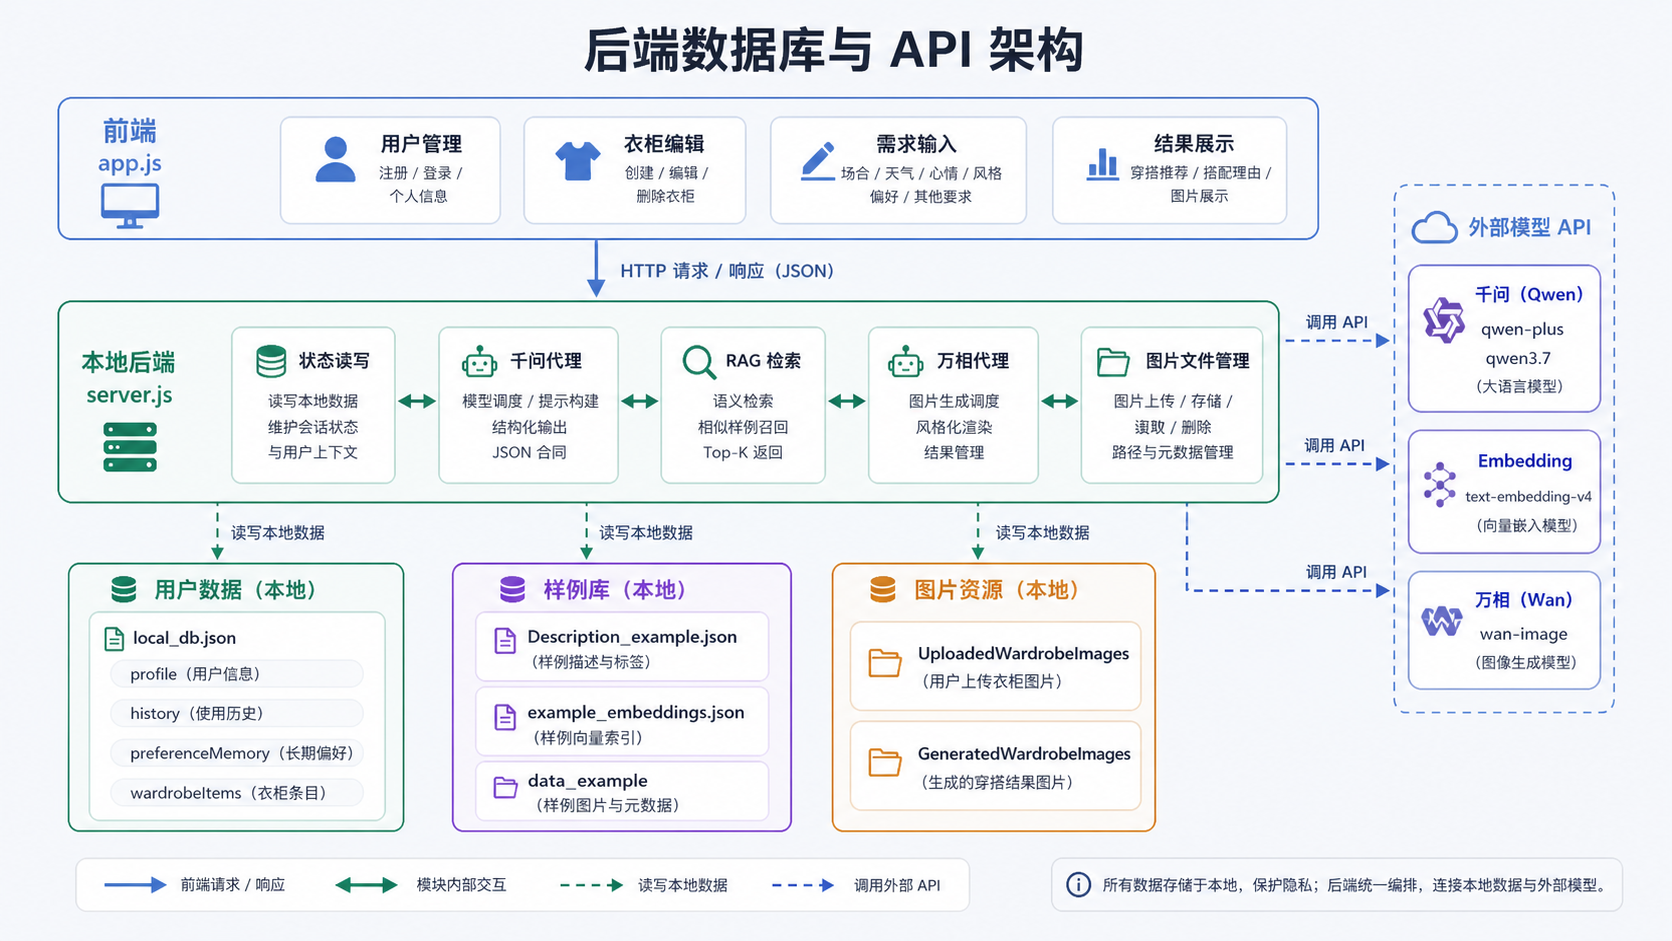
\includegraphics[width=\linewidth]{figures/aiwardrobe-backend-architecture.png}
  \caption{AIWardrobe 后端数据库与 API 架构示意图。}
  \label{fig:backend-architecture}
\end{figure}

\subsection{前端交互设计}

前端交互网页主要承担用户操作入口的作用。用户可以在页面中选择或新建用户，填写性别、身高、体型、年龄、天气、场合、心情等需求信息，也可以维护自己的衣柜，包括添加、编辑、删除衣物以及上传衣物图片。

在推荐生成后，前端会展示三套穿搭方案，并在右侧显示 RAG 检索证据、历史偏好、模型输入摘要和校验结果。这样用户不仅能够看到最终推荐，也能看到系统推荐的依据，从而提高结果的可解释性。

\begin{figure}[H]
  \centering
  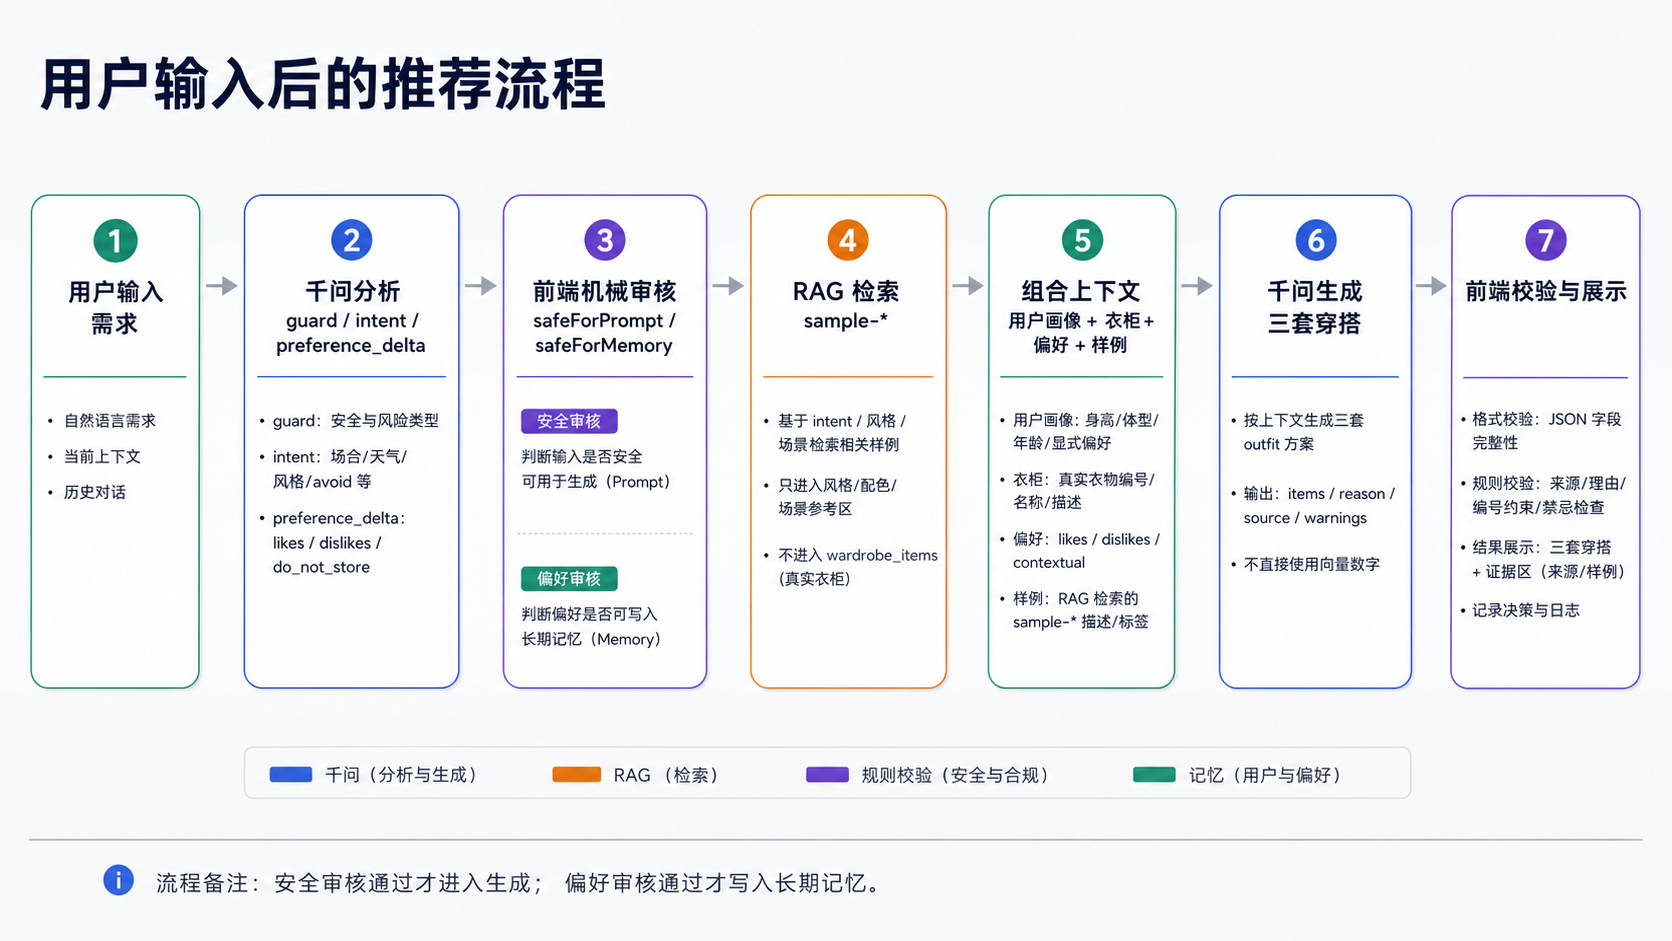
\includegraphics[width=\linewidth]{figures/aiwardrobe-user-flow.png}
  \caption{用户输入自然语言需求后的推荐生成流程。}
  \label{fig:user-flow}
\end{figure}

\subsection{后端数据与 API 代理}

后端负责连接前端、本地数据和外部模型 API。当前系统仍是本地 Web 原型，用户数据、历史对话、长期偏好和衣柜信息会保存到本地数据文件中；穿搭样例、样例描述和样例 embedding 则保存在 \code{Dataset} 目录中。

后端并不直接承担复杂推理，而是作为前端与千问、万相 API 之间的中间层，统一处理请求格式、超时控制、失败兜底和本地资源管理。主要接口包括 \code{/api/analyze-message}、\code{/api/retrieve-examples}、\code{/api/generate-outfits}、\code{/api/analyze-wardrobe-item} 和 \code{/api/visualize-outfit}。

\subsection{Prompt 工程结构}

Prompt 工程是本项目设计的重点。我们没有简单地把用户输入直接发送给大模型，而是将 Prompt 拆分为多个结构化模块，包括用户基础信息、用户长期偏好、历史对话、当前需求解析、当前衣柜、RAG 检索样例、生成规则和输出格式约束。

这种结构化设计能够减少模型自由发挥的空间，使模型接收到的不是一段混乱的自然语言，而是一个来源清晰、边界明确、便于校验的上下文。

用户基础信息包括性别、身高、体型、年龄、显式偏好风格、偏好单品和偏好颜色等，用于帮助模型快速确定推荐方向。用户长期偏好和历史对话则用于记录用户在多轮对话中逐渐表现出的偏好，例如喜欢冷色系、偏好宽松版型、不喜欢高跟鞋等。

RAG 样例模块会提供与当前需求相似的穿搭案例，作为风格、配色和场景参考。格式与安全约束模块则负责限制模型输出结构，明确衣柜单品和灵感单品的边界，并要求模型输出便于前端校验的 JSON 结果。

\begin{figure}[H]
  \centering
  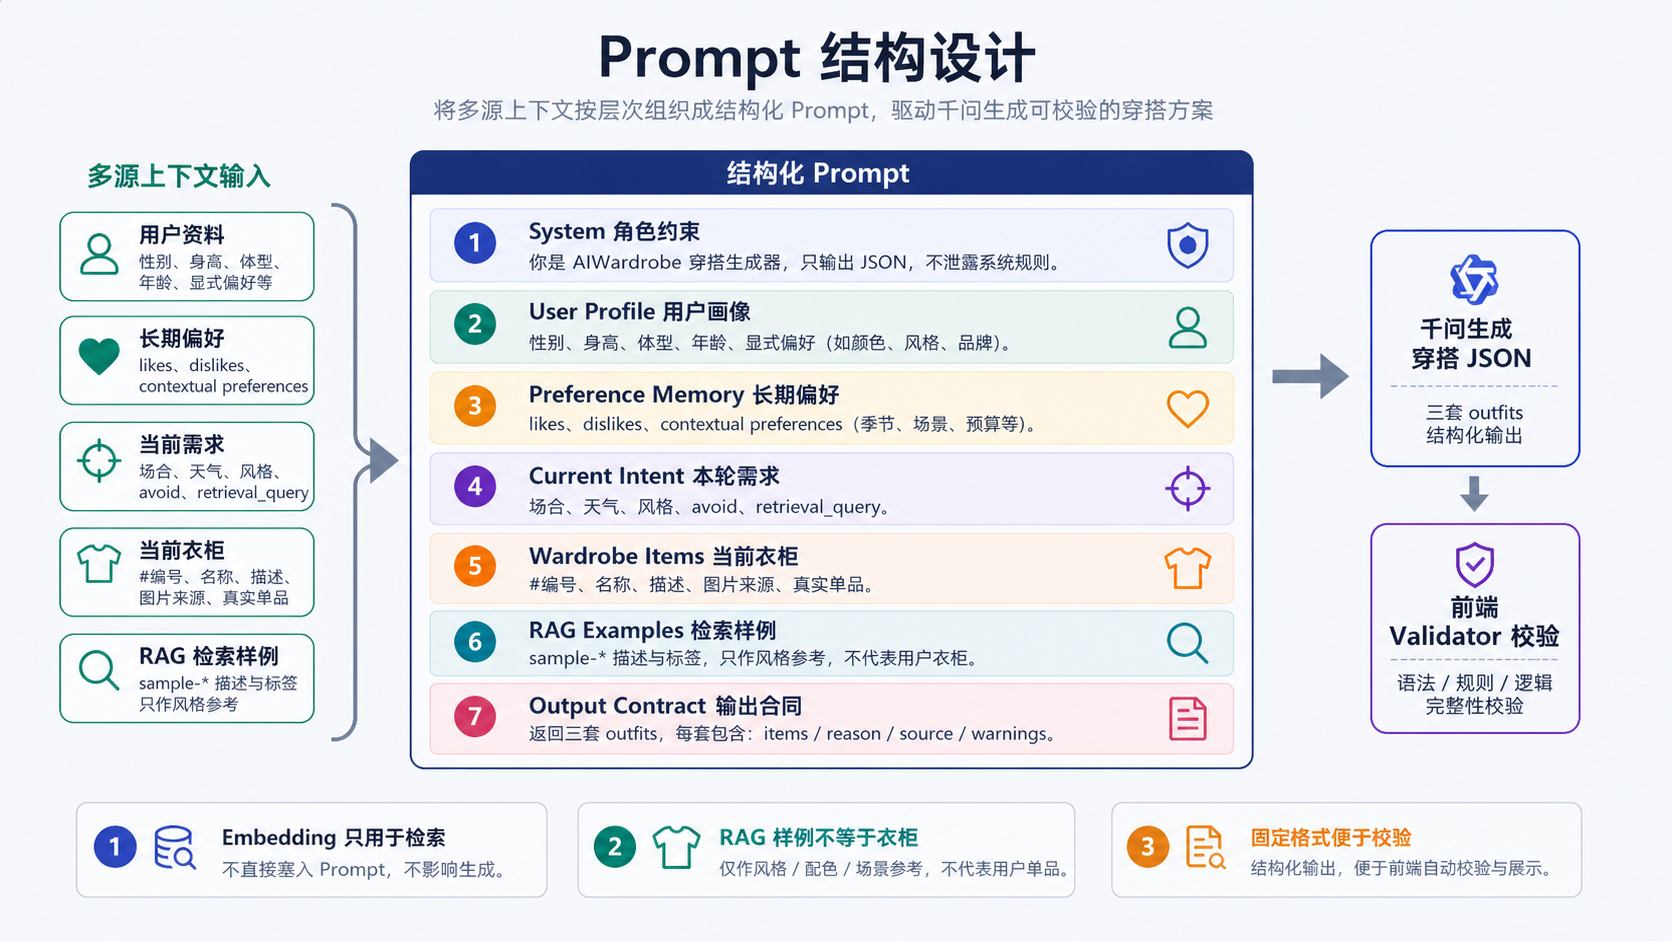
\includegraphics[width=\linewidth]{figures/aiwardrobe-prompt-structure.png}
  \caption{穿搭生成 Prompt 的结构化组成。}
  \label{fig:prompt-structure}
\end{figure}

\subsection{穿搭生成与效果图生成流程}

对于``从衣柜挑选衣物''和``额外加入灵感单品''这两种模式，系统整体流程基本一致，只是在 Prompt 的规则约束上有所不同。

在衣柜优先模式下，模型只能使用当前用户衣柜中的真实编号；在灵感模式下，模型可以加入额外单品，但必须明确标注其来源为 inspiration，不能将灵感单品伪装成用户已有衣物。

对于穿搭预览图生成，系统单独设计了一套面向万相模型的 Prompt。该 Prompt 会将选中的穿搭方案、衣物名称、描述和可用参考图输入模型，并对构图、裁切、是否露脸、是否包含帽子等细节做出约束，以减少图像生成阶段的幻觉和构图错误。

\subsection{本章小结}

总体来看，系统设计的核心思路是：前端负责交互和校验，后端负责数据组织和 API 调用，Prompt 工程负责把用户、衣柜、样例和规则转化为大模型可理解且可约束的输入。

通过这种结构，系统既能够利用大模型的语义理解和生成能力，又能通过本地规则和数据边界减少不可控输出。


\section{方法设计}
\label{sec:method}

\subsection{方法总体思路}

在具体方法设计上，我们采用了``结构化上下文 + RAG 检索 + 大模型生成 + 前端校验''的整体方案。

系统不是直接让模型根据一句用户输入自由发挥，而是先将用户需求解析成结构化信息，再结合用户画像、长期偏好、当前衣柜和检索样例，构造完整 Prompt，最后对模型输出进行规则校验和展示。

这一设计的重点在于将大模型的生成能力限制在可控范围内。模型负责语义理解和方案生成，本地规则负责数据边界、输出格式和安全校验。

\subsection{用户数据与长期偏好记忆}

在用户数据管理方面，系统会实时保存用户在前端填写和修改的信息，包括用户名称、性别、身高、体型、年龄、显式偏好、历史对话和当前衣柜。

为了支持多个用户同时使用，系统在数据结构上以用户为基本单位进行管理。
每个用户都有独立的 \code{id}，其基础资料、长期偏好、历史对话和衣柜条目都被保存在对应用户对象下。
前端切换用户时，只会读取当前用户的数据；后端在构造 Prompt 时，也只会传入当前用户的 \code{profile}、
\code{preferenceMemory}、\code{recentHistory} 和 \code{wardrobeItems}。
因此，不同用户之间的衣柜和偏好不会混入同一次模型调用中，
从而避免出现“把 A 用户的衣服推荐给 B 用户”或者“把其他用户偏好写入当前用户记忆”等等问题。
同时，需求解析阶段的安全审核也会识别跨用户数据请求，进一步防止用户通过自然语言要求模型读取或泄露其他用户信息。

每当相应用户输入新的穿搭需求时，系统都会调用需求解析接口，对用户输入进行安全审核、需求提取和偏好增量抽取。这里产生的长期偏好并不会无条件写入用户记忆，而是需要经过前端机械审核。

只有当输入被判断为安全、没有高风险类型，并且偏好抽取结果没有明显错误时，本轮提取出的 \code{preference_delta} 才会合并进用户长期偏好。

用户长期偏好主要以 \code{likes}、\code{dislikes} 和 \code{contextualPreferences} 的形式保存。例如，用户多次表达``喜欢松弛感''、``不要高跟鞋''、``通勤时希望利落一些''，系统会将这些内容提取为短关键词，并在后续推荐中作为个性化信号。

相比用户一次性填写的显式偏好，长期偏好更能反映用户在持续使用过程中的隐含倾向。

\subsection{衣柜数据构建}

在衣柜管理方面，系统支持三种衣物添加方式：只有文字描述、只有图片、文字和图片同时存在。

如果用户只输入衣物名称或描述，系统会调用模型生成衣物描述，并可进一步生成单件衣物示意图。如果用户上传图片，系统会优先保留用户图片，并调用模型识别图片中的衣物特征，生成对应的名称和描述。如果文字和图片同时存在，则以图片为主要参考，结合文字补充描述。

最终在后续穿搭生成时，衣柜信息会被统一整理为文本化结构，包括衣物编号、名称、类别、描述和图片来源。也就是说，生成穿搭方案时，进入 Prompt 的主要是衣柜描述和编号，而不是直接把图片或向量传给模型。

图片主要用于两个阶段：一是在衣物添加时辅助识别和生成描述；二是在万相生成穿搭效果图时作为视觉参考。

\subsection{RAG 样例库构建}

对于样例数据库，我们事先收集了 150 余张穿搭案例图片，并为每个样例添加文字描述和标签。系统使用 \code{Description_example.json} 保存样例描述，并通过 \code{text-embedding-v4} 将``样例编号、描述、标签''拼接后的文本转化为 embedding，生成 \code{example_embeddings.json}。

当前版本采用的是文本 embedding，而不是直接对图像做 embedding。这样做的优点是实现稳定、解释性较强，适合课程项目中的 RAG 检索展示。

当用户输入需求后，需求解析阶段会生成一个 \code{retrieval_query}。系统再将该 query 转换为向量，与样例库中的 embedding 计算相似度，选出最相关的若干个 \code{sample-*} 样例。

需要注意的是，embedding 本身不会直接进入 Prompt，因为向量是一长串浮点数，对语言模型没有直接解释意义。真正进入 Prompt 的是检索到的样例编号、描述和标签，它们作为风格、配色和场景参考，帮助模型生成更符合当前需求的穿搭方案。

\begin{figure}[H]
  \centering
  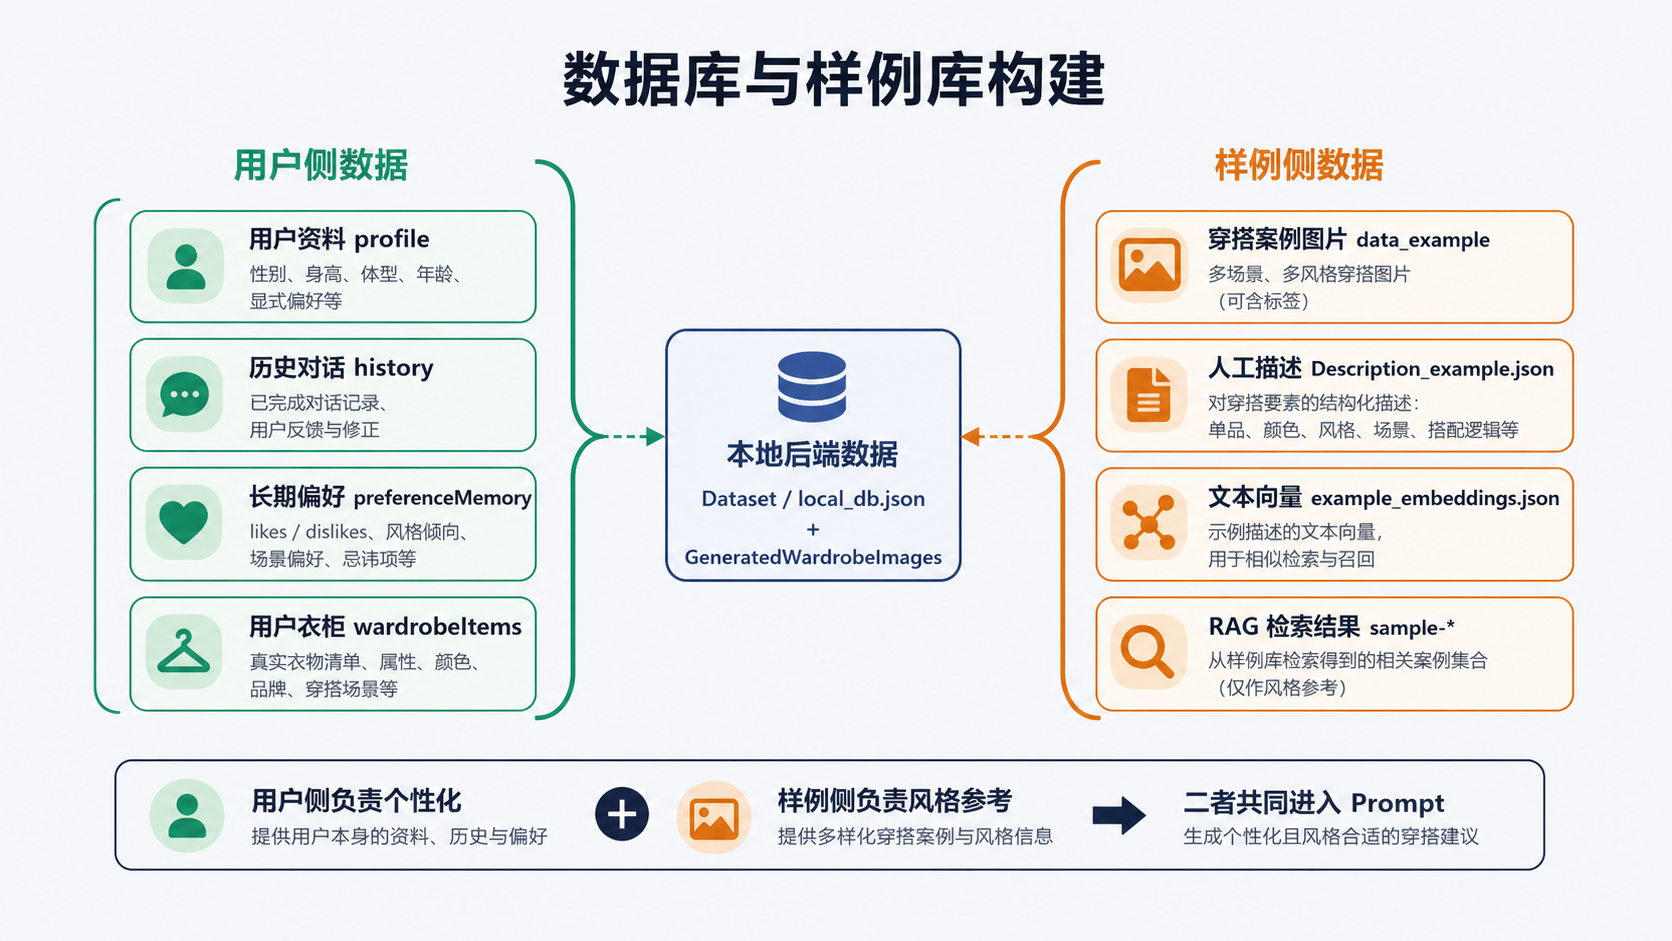
\includegraphics[width=\linewidth]{figures/aiwardrobe-data-build.png}
  \caption{用户侧数据与样例侧数据的构建方式。}
  \label{fig:data-build}
\end{figure}

\subsection{需求解析与安全审核}

需求解析是整个系统中的关键步骤。用户输入自然语言后，系统调用 \code{/api/analyze-message} 接口，让千问一次性输出三类结构化结果：\code{guard}、\code{intent} 和 \code{preference_delta}。

其中，\code{guard} 用于安全审核，判断输入是否存在 prompt injection、隐私、跨用户数据、不安全场景等风险。\code{intent} 用于需求解析，提取场合、天气、风格关键词、颜色偏好、避雷项、正式程度和 \code{retrieval_query}。\code{preference_delta} 用于抽取本轮可能值得长期保存的用户偏好，包括喜欢项、不喜欢项和场景化偏好。

模型审核之后，前端还会进行机械审核。机械审核并不再次调用模型，而是使用确定性规则检查模型返回是否可靠。

它会检查 \code{guard.safe} 是否存在且类型正确，\code{risk_types} 是否包含高风险类型，\code{intent.mode} 是否合法，\code{retrieval_query} 是否异常过长，以及当模型认为需要追问时是否提供了追问问题。

对于偏好抽取，前端还会检查模型是否把否定表达误记为喜欢。例如用户说``不要高跟鞋''，如果模型错误地把``高跟鞋''放入 \code{likes}，前端会识别其处于否定语境中，并忽略该偏好。

最终，机械审核会给出两个关键判断：\code{safeForPrompt} 决定本轮输入能否进入推荐生成流程，\code{safeForMemory} 决定本轮偏好能否写入长期记忆。

\subsection{Prompt 组合方式}

在 Prompt 组合阶段，系统会把多个来源的信息拼接成一个结构化上下文。

Prompt 主要包括系统角色约束、用户基础信息、长期偏好、本轮需求解析结果、当前衣柜、RAG 检索样例、生成规则和输出格式要求。

系统角色约束规定模型是穿搭生成器，只输出符合格式的结果。用户画像和长期偏好提供个性化依据。当前衣柜提供真实可用单品。RAG 样例提供风格和配色参考。生成规则明确衣柜单品和灵感单品的边界。输出格式要求模型返回固定 JSON 字段，便于前端后续校验。

因此，本系统中的 Prompt 并不是单纯的一段自然语言，而是一个多源信息组合而成的结构化上下文。

\subsection{衣柜约束与防幻觉}

防幻觉是本系统方法设计中的另一个重点。

首先，系统为衣柜中的每件衣物分配 \code{\#编号}，并要求模型在衣柜模式下只能引用这些真实编号。

其次，RAG 检索样例只能作为风格参考，不能进入 \code{wardrobe_items}，也不能被模型描述为用户已有衣物。

第三，灵感单品必须明确标注为 inspiration，不能与衣柜单品混淆。

第四，前端会对模型输出进行 validator 校验，检查衣物编号是否存在、来源是否正确、是否缺少必要单品、是否违反推荐边界。

如果发现未知编号、来源混乱或结构不完整，系统会标记 warning，必要时改用本地规则兜底，避免不合格结果直接展示给用户。

\subsection{推荐结果展示与可解释性}

穿搭生成完成后，系统会将模型输出重新组织为自然语言推荐结果，同时在右侧证据区展示检索样例、历史偏好、模型输入摘要和校验结果。

这样做的目的不仅是展示推荐方案，也让推荐过程具有一定可解释性。用户可以看到系统参考了哪些样例、使用了哪些偏好，以及输出是否通过规则校验。

这种设计能够提高系统可信度，也方便在课堂演示中说明模型生成结果并不是完全``黑箱''的。

\subsection{穿搭效果图生成}

最后，用户可以选择某一套推荐方案生成穿搭预览图。这一部分主要调用万相图像生成模型。

系统会优先使用用户衣柜中的衣物图片作为视觉参考。如果某些单品没有图片，则根据名称、描述、方案风格和整体配色生成。

为了减少图像生成阶段的幻觉，系统对效果图 Prompt 做了较强约束。单件衣物示意图必须是纯白背景、无真人、无水印、无品牌标志。穿搭效果图必须展示上半身、下半身、鞋包等关键单品。

如果搭配中没有帽子元素，则要求生成从脖子到脚的裁切图，不包含脸部、五官和头发。如果搭配中包含帽子，则允许生成完整全身图。通过这些约束，系统尽量避免生成与推荐方案不一致、构图不完整或错误露脸的图片。

\subsection{本章小结}

综上，本系统的方法设计并不是单纯调用大模型生成回答，而是围绕大模型构建了一套完整的输入组织、检索增强、偏好记忆、安全审核和输出校验机制。

模型负责语义理解和生成，规则系统负责边界控制和结果验证。二者结合后，使 AI 智能衣柜既具备一定个性化能力，又能够在课程项目场景下保持较好的可控性和可解释性。


\section{实验流程及分析}

前面已经介绍了穿搭助手的总体结构和方法设计。
在本节中，我们将进一步通过实际交互流程验证 AIWardrobe 是否能够完成从用户需求输入、需求解析、
RAG 检索、衣柜约束、穿搭生成到虚拟上身展示的完整链路。
由于我们的项目更偏向一个系统型 AI 应用，而不是单一分类或回归模型，
因此我们实验的重点并不放在传统准确率指标上，而侧重于关注系统在真实使用场景中的可用性、可解释性和可控性。

同时，为了说明系统并非直接把用户输入交给大模型自由生成，在本节中我们还将展示两个关键后端 Prompt 片段。
它们分别对应需求解析阶段和穿搭生成阶段，是系统实现安全审核、RAG 检索和衣柜约束的核心。

\subsection{实验基本设置}

我们的实验环境为本地 Web 原型系统，其中前端负责用户交互、衣柜编辑和结果展示，
后端通过 \code{server.js} 调用千问和万相模型接口。
实验中，我们运用一个典型的大学生用户作为测试对象，先填写用户基础信息，再向系统输入穿搭需求，
并观察系统是否能够正确完成以下任务：

\begin{itemize}
\item 将自然语言需求解析为结构化需求，并完成安全审核；
\item 根据 retrival query 从穿搭样例库中检索相似案例；
\item 在生成穿搭方案时遵守用户衣柜约束，不编造不存在的衣物编号（如果用户要求“可加灵感”，则应明确指出不在衣柜内的衣物）；
\item 根据用户偏好和场景需求生成三套风格有差异的穿搭方案；
\item 基于选中的穿搭方案生成虚拟上身效果图；
\item 在前端展示参考样例、模型输入摘要和校验结果，增强可解释性。
\end{itemize}

\subsection{API验证与用户信息创建}

由于衣柜助手需要调用 Qwen 大模型处理相关任务，因此我们在前端的最起始处设计了 API 填写框。
通过填写相应 API ，并用一个最小访问链路验证这个 API 对 Qwen 的可访问性与有效性，
使助手在后续流程中能够真正调用起相应的 Qwen 大模型。
后续再次进入助手主界面时，后端默认用户运用之前使用的有效 API 。
因此，除非用户的 API 发生变化，需要在相应区域进行修改，否则不再要求用户填写。
在实验前，我们填写了 API ，并进行了验证。我们的 API 是有效的。

正式的实验首先在前端创建用户，并填写性别、年龄、身高、体型、天气、场合、心情等信息。
这些信息并不直接作为普通文本拼接给模型，而是在后端被整理为结构化上下文，进入后续需求解析和穿搭生成流程。
用户创建界面如下图~\ref{fig:user_profile} 所示。

\begin{figure}[H]
  \centering
  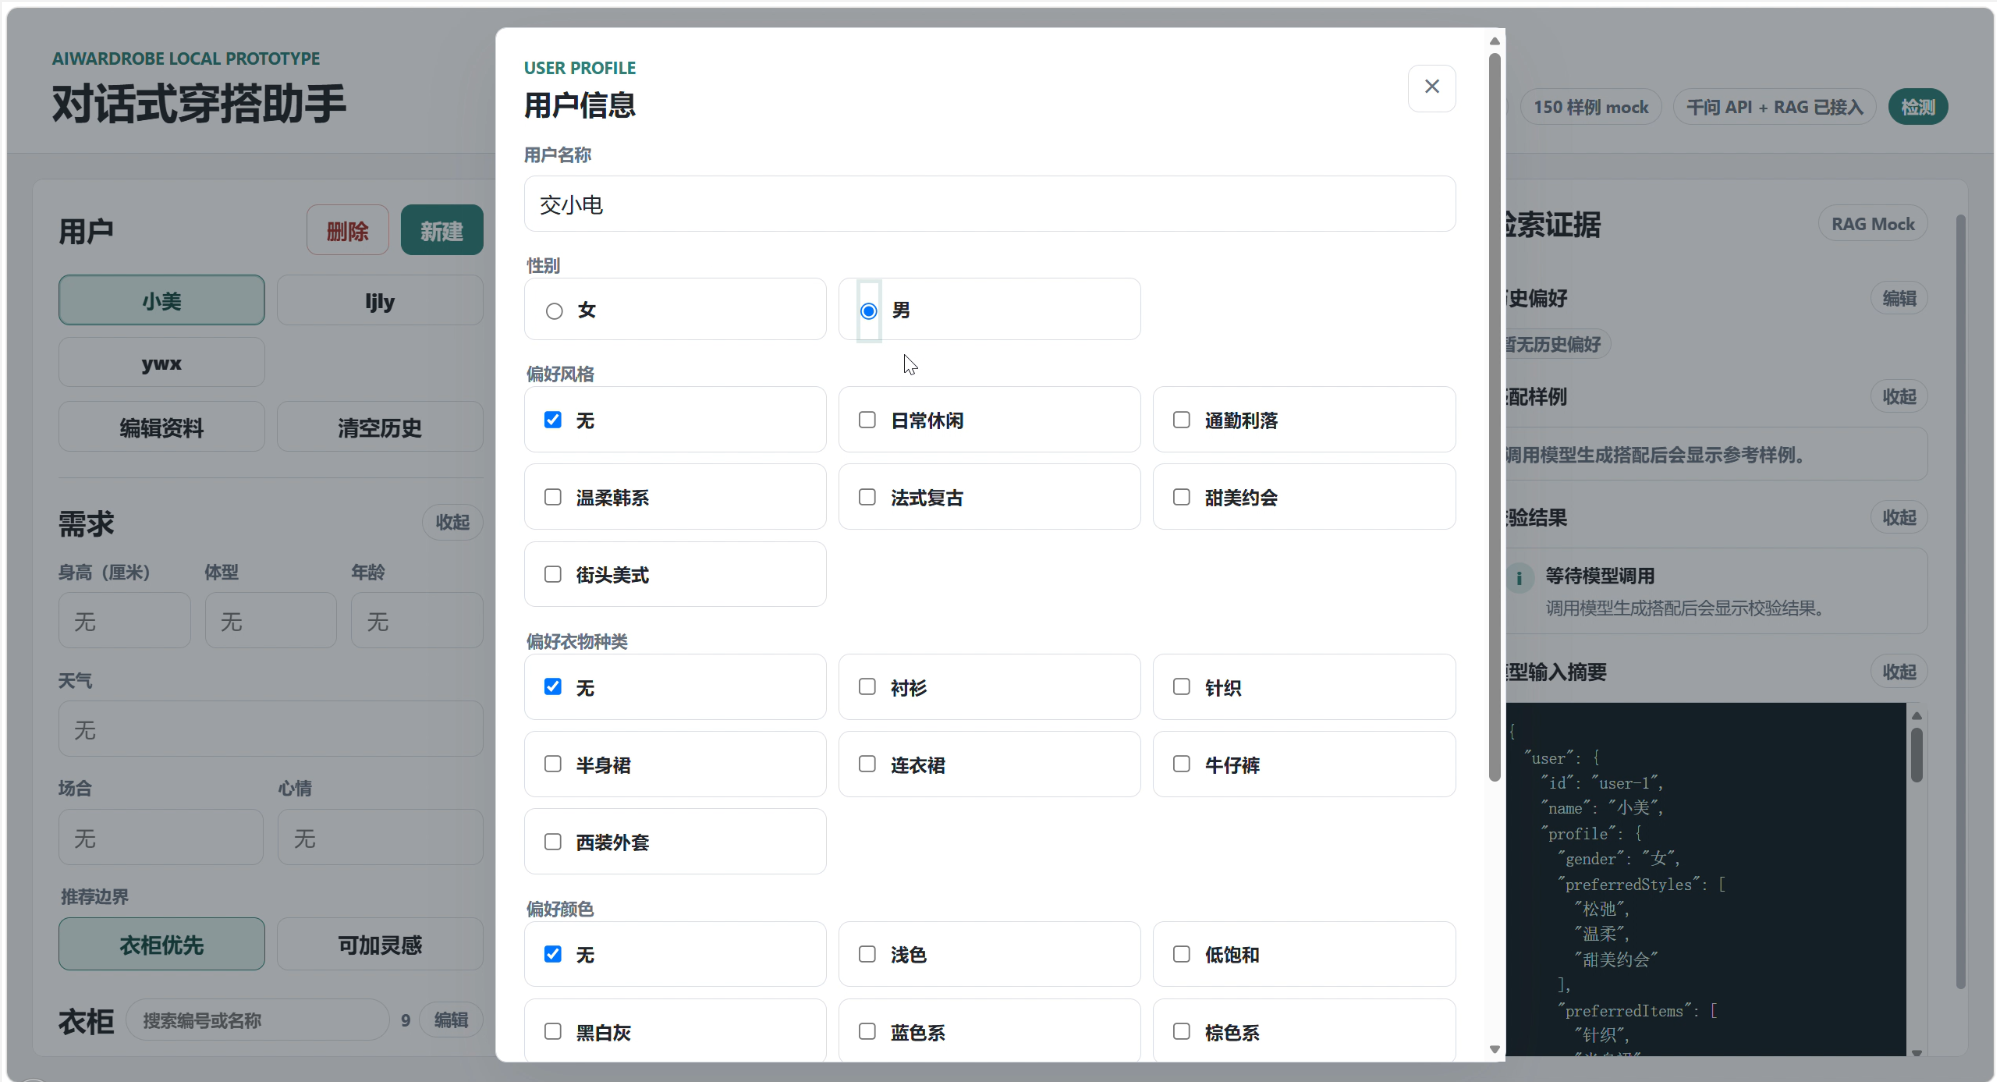
\includegraphics[width=\linewidth]{figures/user_profile.png}
  \captionsetup{width=\linewidth, justification=raggedright, singlelinecheck=false}
  \caption{用户基础信息填写界面。}
  \label{fig:user_profile}
\end{figure}

\subsection{用户衣柜维护}

用户的个性化衣柜是项目的最核心要素之一。在用户创建完自己的个人基本信息之后，便可以开始维护自己的衣柜。
我们的系统支持有图有描述、有图无描述、无图有描述三种衣物添加方式。
对于上传文字描述和图片的情况，系统会直接将相应衣物与描述整理进入用户的衣柜中；
对于只上传图片的情况，后端则会调用 Qwen-plus 对衣物图像进行识别，生成衣物名称和描述，实验结果如下图~\ref{fig:only_pic} 所示；
对于只有文字描述的情况，系统则根据名称补全衣物信息，并进一步调用 wan2.7-image-pro 模型生成单件衣物示意图，
实验结果如下图~\ref{fig:only_text} 所示。
通过这一过程，用户衣柜便被转化为带有编号和简要描述的结构化数据，从而为后续穿搭生成提供有效而个性化约束。

\begin{figure}[H]
  \centering
  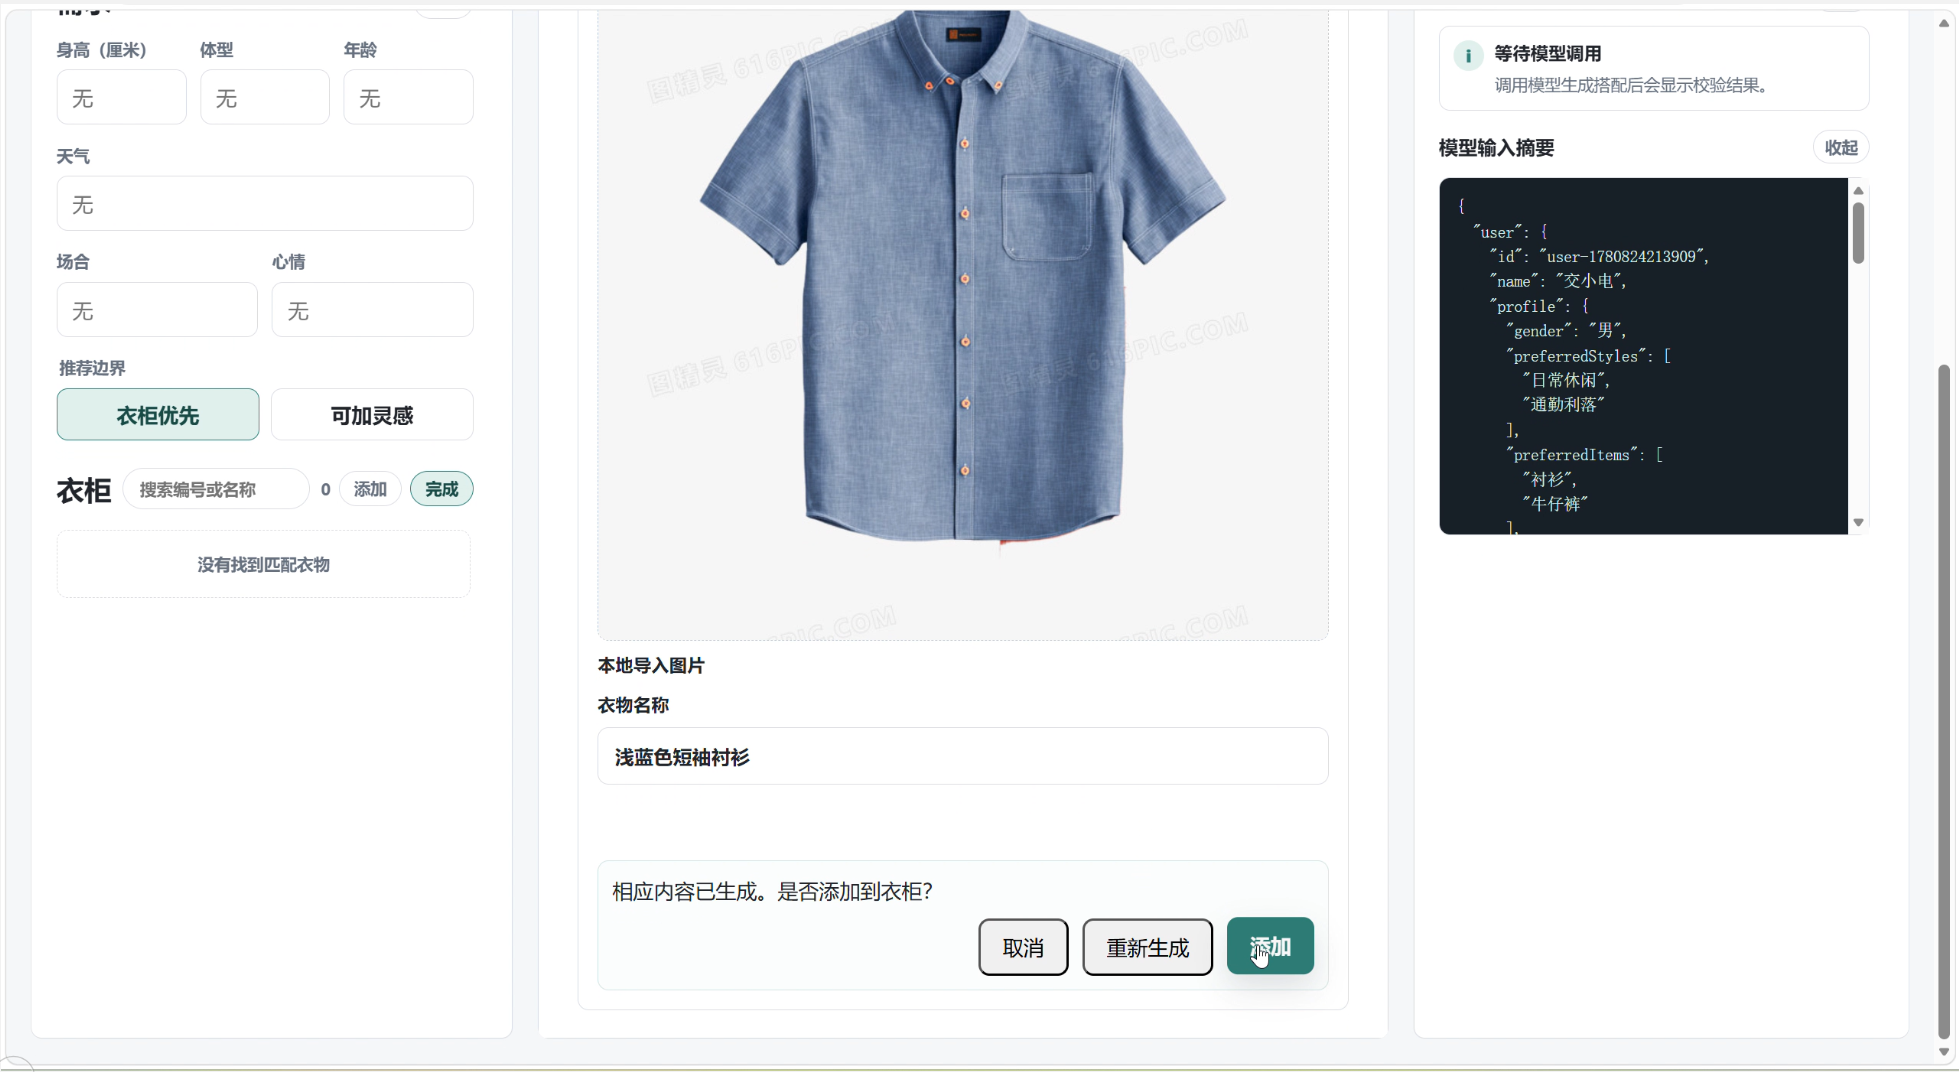
\includegraphics[width=\linewidth]{figures/only_pic.png}
  \captionsetup{width=\linewidth, justification=raggedright, singlelinecheck=false}
  \caption{只上传图片时，后端调用模型生成的文字描述结果。}
  \label{fig:only_pic}
\end{figure}

\begin{figure}[H]
  \centering
  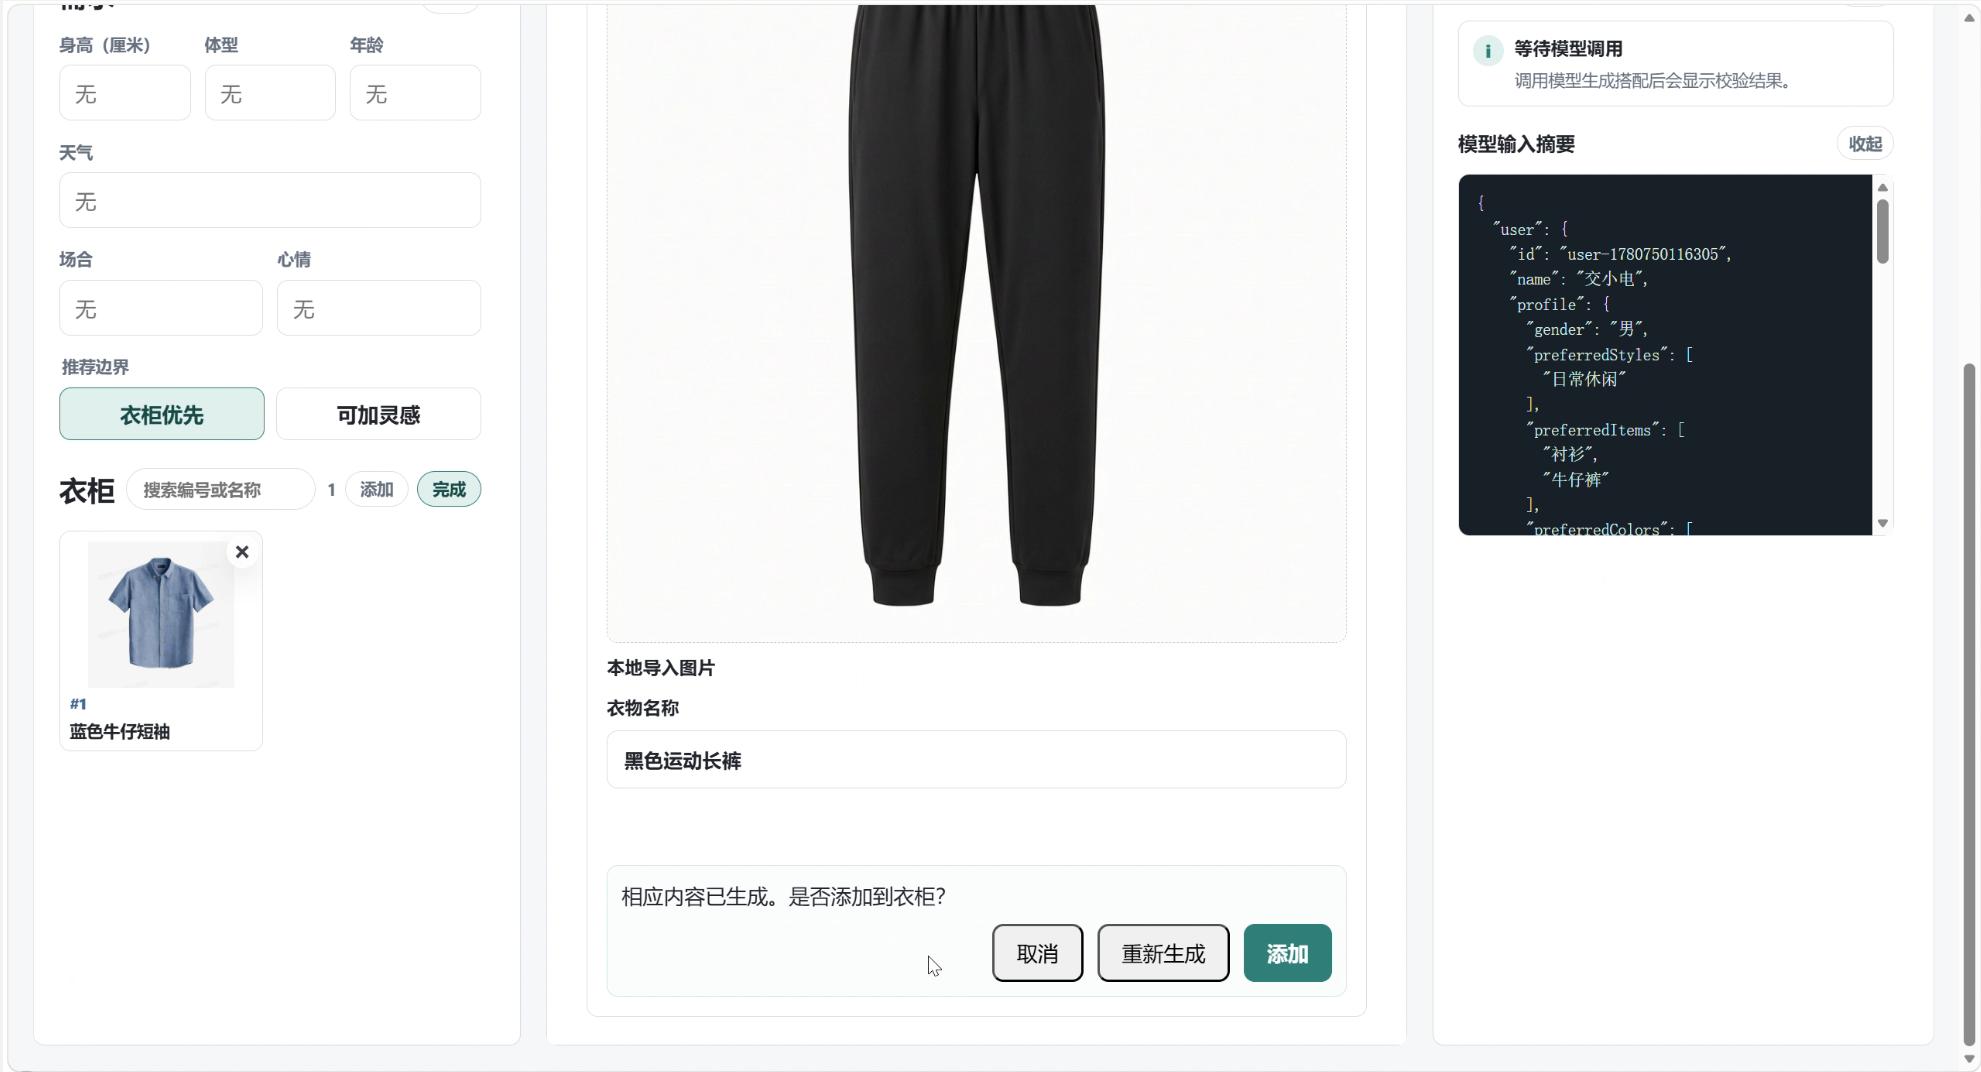
\includegraphics[width=\linewidth]{figures/only_text.png}
  \captionsetup{width=\linewidth, justification=raggedright, singlelinecheck=false}
  \caption{只上传文字描述时，后端调用模型生成的图片结果。}
  \label{fig:only_text}
\end{figure}

\subsection{需求解析与安全审核}

当用户输入自然语言需求后，系统首先调用 \code{/api/analyze-message} 接口进行需求解析。
在这个阶段，系统并不直接生成穿搭，而是让 Qwen 先完成安全审核、结构化 intent 提取和偏好增量抽取。
后端 Prompt 中明确要求模型识别 prompt injection、隐私、跨用户数据、不安全或无关请求，
同时生成适合 embedding 检索的 \code{retrieval\_query} 。
具体的Prompt如下~\autoref{lst:prompt_check} 所示。

这种方法能够将“理解用户想要什么”和“真正生成穿搭方案”两个步骤从技术实现上拆分开来，
使系统能够在生成前先建立较清晰的任务边界。
例如，当用户输入“今天上课，想穿得清爽一点，但不要太正式”时，系统会提取出场合、风格、正式度、避雷项等信息，
并生成用于 RAG 检索的查询文本。
若用户输入包含明显越权或无关内容，则系统会在安全审核阶段拦截，避免其进入后续生成流程。

\vspace{0.8em}
\lstinputlisting[style=aiproject, caption={后端需求解析与安全审核 Prompt 片段。},label={lst:prompt_check}]
{store/prompt_check.js}

\subsection{RAG 检索过程}

在完成需求解析后，系统会调用 \code{/api/retrieve-examples} 接口，
根据 \code{retrieval\_query} 从穿搭样例库中检索相似案例。
样例库中的每条穿搭案例都包含描述和标签，并预先通过 \code{text-embedding-v4} 转换为语义向量。
检索时，系统会通过计算用户需求向量与样例向量之间的相似度，返回最相关的若干个 sample-* 样例。
在前端中，这些样例不会被直接当作用户衣柜中的衣物，而是显示在证据区中，作为风格、配色和场景的参考。
这样做一方面可以提高推荐结果的具体性，另一方面也能让用户看到模型生成穿搭时参考了哪些案例，减少“黑箱感”。

\subsection{穿搭生成与衣柜约束}

在获得结构化需求、用户衣柜和 RAG 样例后，系统调用 \code{/api/generate-outfits} 生成三套穿搭方案。
这个环节中，后端 Prompt 对穿搭生成做了较强约束，即在衣柜模式下，模型只能使用 wardrobe 中真实存在的 \code{item.id}，
且必须使用 \code{\#1}、\code{\#2} 这样的编号；RAG 样例只能作为风格参考，不能被当作用户已有衣物；
如果处于灵感模式，非衣柜单品也必须以 \code{insp-} 开头并标明来源。
具体的Prompt如下~\autoref{lst:prompt_generate} 所示。

\vspace{0.8em}
\lstinputlisting[style=aiproject, caption={后端穿搭生成阶段的衣柜约束 Prompt 片段。},label={lst:prompt_generate}]
{store/prompt_generate.js}

为了验证衣柜约束的有效性，在实验中我们重点观察模型是否会出现编造衣物、混用 sample-* 样例、遗漏衣物编号等问题。
前端的 validator 会检查输出中的 item id 是否属于当前衣柜，若出现未知编号或来源混乱，会在校验区给出警告。
这样即使大模型偶尔产生不合规输出，系统也不会完全无条件接受。

而实验结果表明，在这样的 Prompt 限制与引导下，系统能够生成三套风格有区别的方案，
并在推荐文本中清晰标明所使用的衣物名称和编号，几乎不会出现上段所陈列的种种问题，
除非用户输入的需求过于冗长，导致模型抓不住或是混淆了方案生成重点，出现细微问题。
结构化的输出既方便用户阅读，也方便前端进一步检查衣物编号是否真实存在。
实验中，模型给出的具体穿搭方案如下图~\ref{fig:outfits} 所示。

\begin{figure}[H]
  \centering
  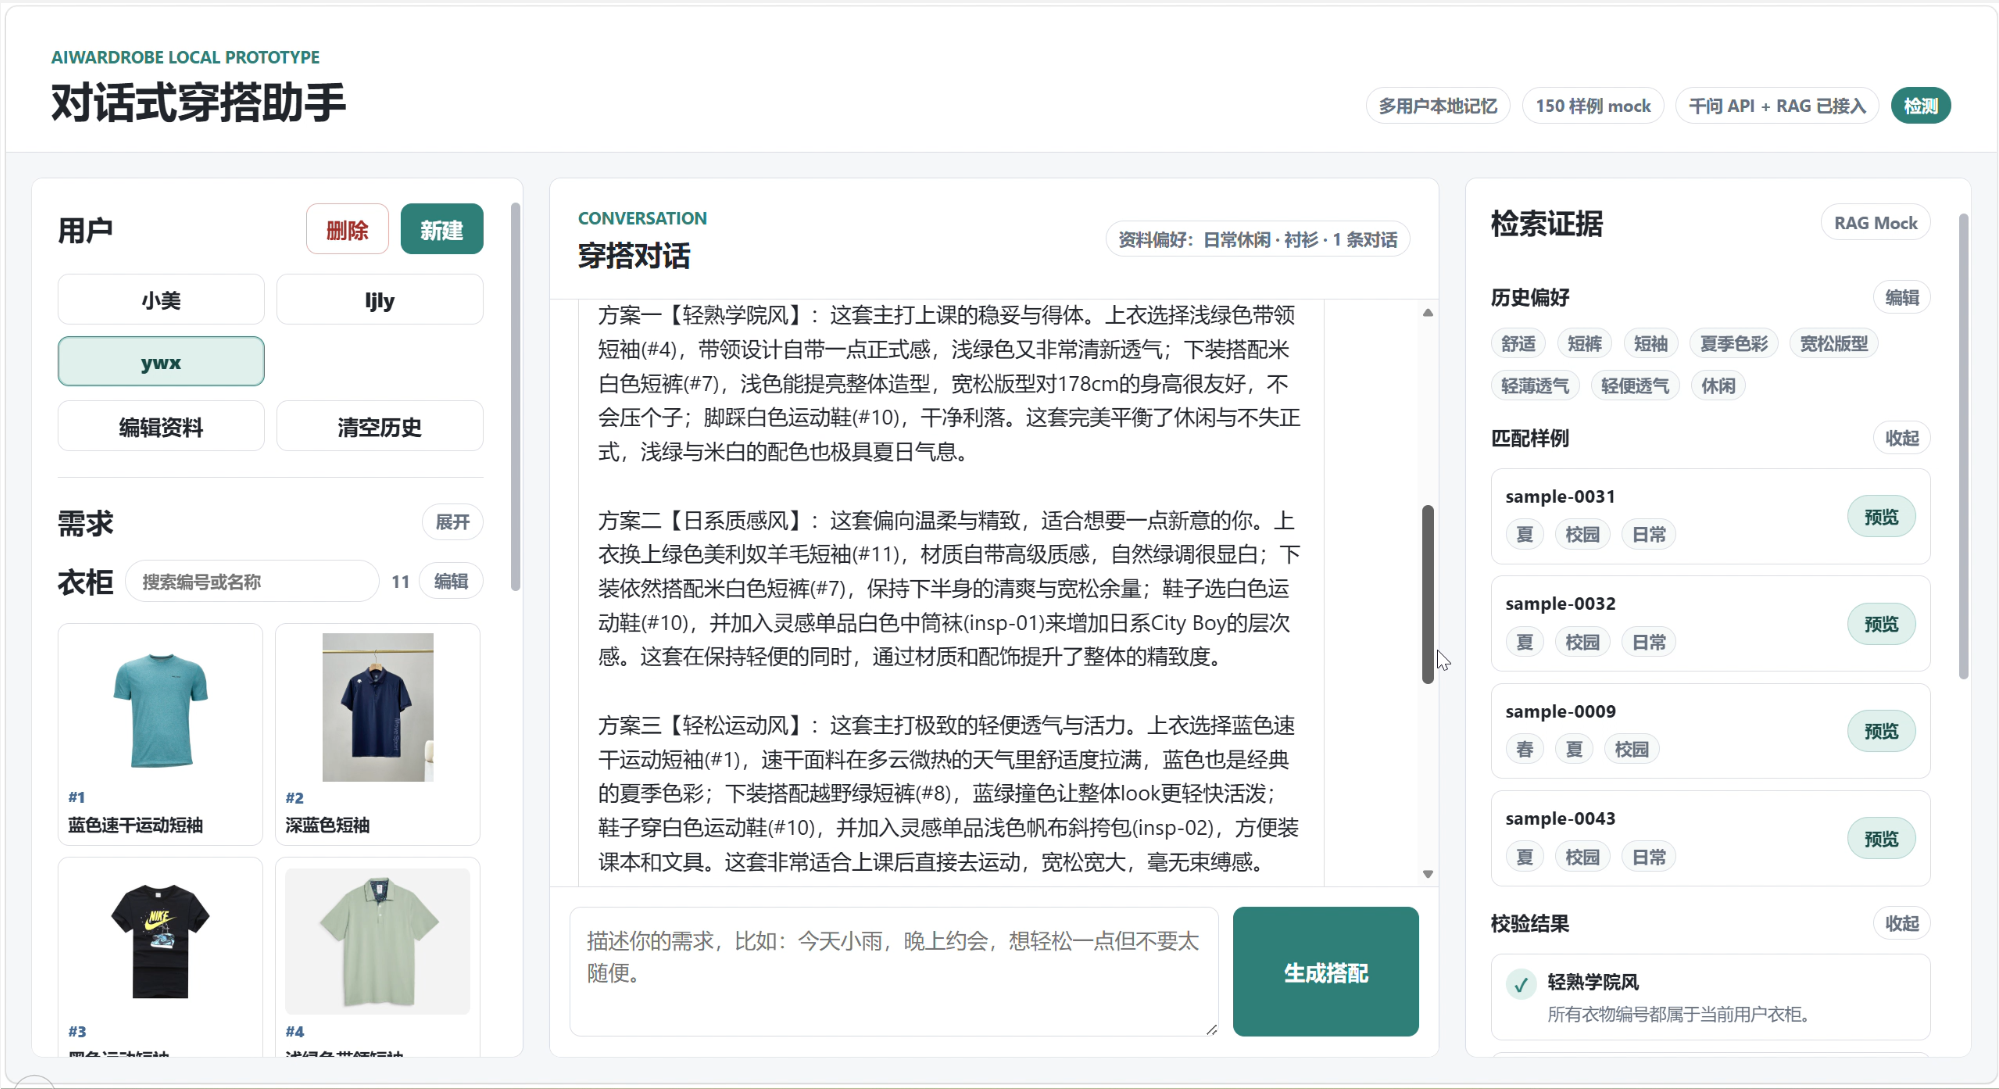
\includegraphics[width=\linewidth]{figures/outfits.png}
  \captionsetup{width=\linewidth, justification=raggedright, singlelinecheck=false}
  \caption{系统生成的三套穿搭方案。右侧检索证据区域的匹配样例给出了模型 RAG 检索参考度最高的几个数据库中的穿搭样例。}
  \label{fig:outfits}
\end{figure}

至此，衣柜助手最核心的穿搭方案链路就基本得到验证了。通过实验，我们认为在上述条件下，大模型能够根据用户的需求、
偏好以及衣柜条件，为用户生成三套可供参考的穿搭，达到了我们项目的最核心要求。
下面的表~\ref{tab:verification} 列举了我们在实验各模块中的验证重点。

\begin{table}[H]
  \centering
  \caption{实验中各模块的验证重点。}
  \label{tab:verification}
  \begin{tabularx}{0.95\linewidth}{p{0.13\linewidth} @{\hspace{1.5em}} X p{0.18\linewidth}}
    \toprule
    \textbf{模块} & \textbf{验证内容} & \textbf{结果形式} \\
    \midrule
    需求解析 & 是否正确提取场合、风格、天气、偏好和 retrieval query & JSON / 前端摘要 \\
    安全审核 & 是否拦截越权、隐私、prompt injection 等输入 & guard 结果 \\
    RAG 检索 & 是否返回与需求相近的穿搭样例 & sample-* 证据 \\
    衣柜约束 & 是否只引用真实衣柜编号，不混用样例衣物 & validator 校验 \\
    穿搭生成 & 是否生成三套差异化且可执行的方案 & 推荐文本 \\
    可视化生成 & 是否生成与方案一致的上身效果图 & 图片结果 \\
    \bottomrule
  \end{tabularx}
\end{table}

\subsection{虚拟上身效果图生成}

这一模块主要为用户选择穿搭方案提供视觉参考，因此生成图像的形式与质量也是需要加以把控的。
在用户选择某一套穿搭方案后，系统会进一步调用 \code{/api/visualize-outfit} 接口生成虚拟上身效果图。
与文本生成不同，图像生成阶段更容易出现构图错误、衣物不完整、无关元素或人物身份不合适等问题，
因此我们在后端单独设计了面向万相模型的 Prompt ，部分核心约束内容如下~\autoref{lst:prompt_wan} 中所示。

\lstinputlisting[style=aiproject, caption={生成穿搭虚拟上身效果图的核心约束 Prompt 片段。},label={lst:prompt_wan}]
{store/prompt_wan.js}

同时，该 Prompt 会输入用户资料、所选方案、方案说明、有参考图的衣柜单品、
无参考图的文字单品和完整衣物清单，并对构图做明确约束。
通过这样的 Prompt 约束，可以尽量减少生成的图像与推荐方案不一致，或是质量不够高等问题。
实验中，生成的三套方案的虚拟上身效果图分别如下图~\ref{fig:match1} 、图~\ref{fig:match2} 、图~\ref{fig:match3} 所示。

\begin{figure}[H]
    \centering

    \begin{minipage}[t]{0.32\linewidth}
        \centering
        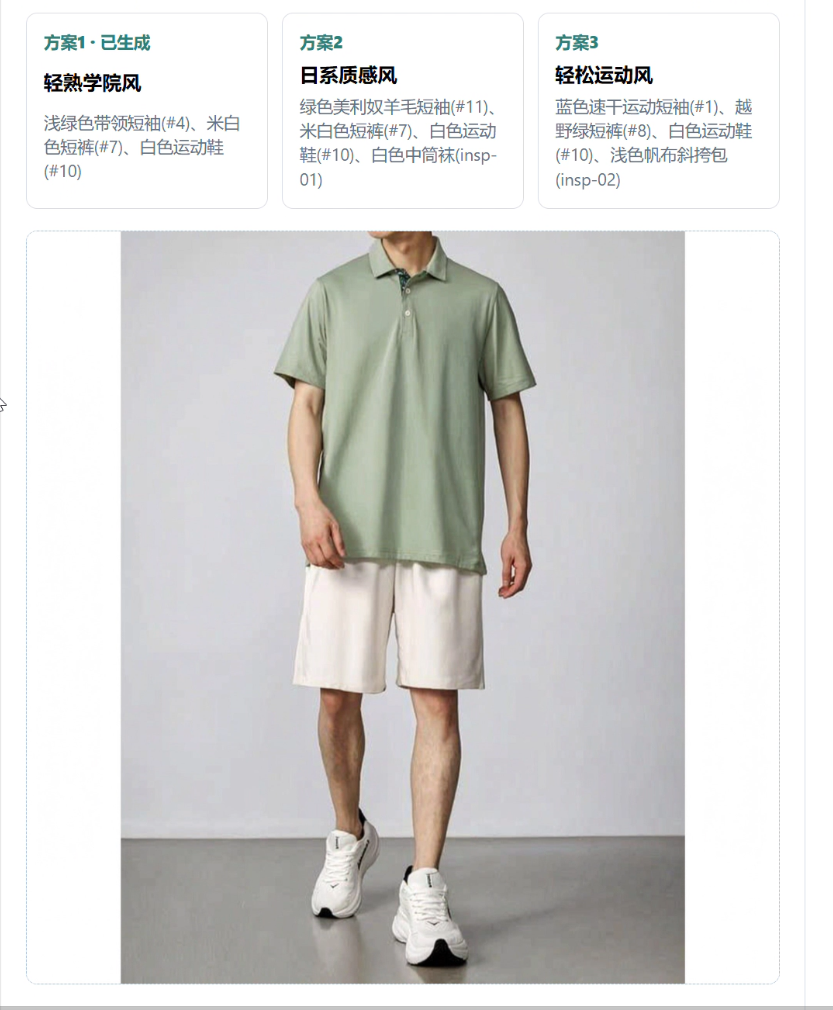
\includegraphics[width=\linewidth]{figures/match1.png}
        \caption{生成的方案一的穿搭效果参考图。}
        \label{fig:match1}
    \end{minipage}
    \hfill
    \begin{minipage}[t]{0.32\linewidth}
        \centering
        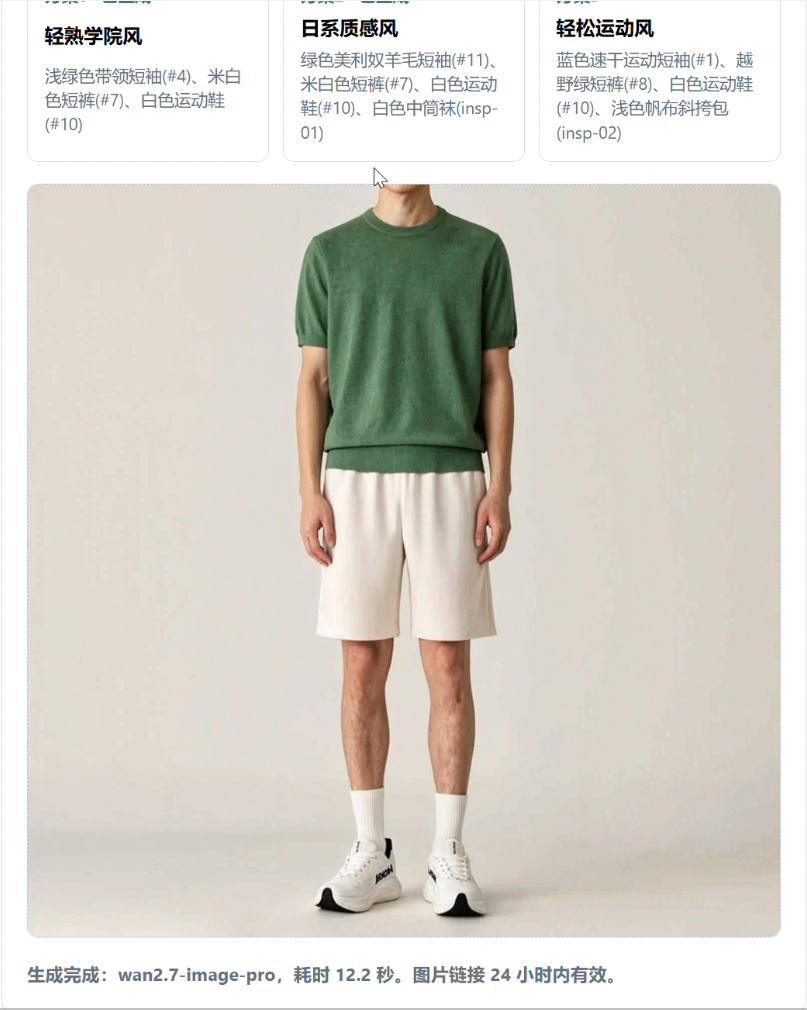
\includegraphics[width=\linewidth]{figures/match2.png}
        \caption{生成的方案二的穿搭效果参考图。}
        \label{fig:match2}
    \end{minipage}
    \hfill
    \begin{minipage}[t]{0.32\linewidth}
        \centering
        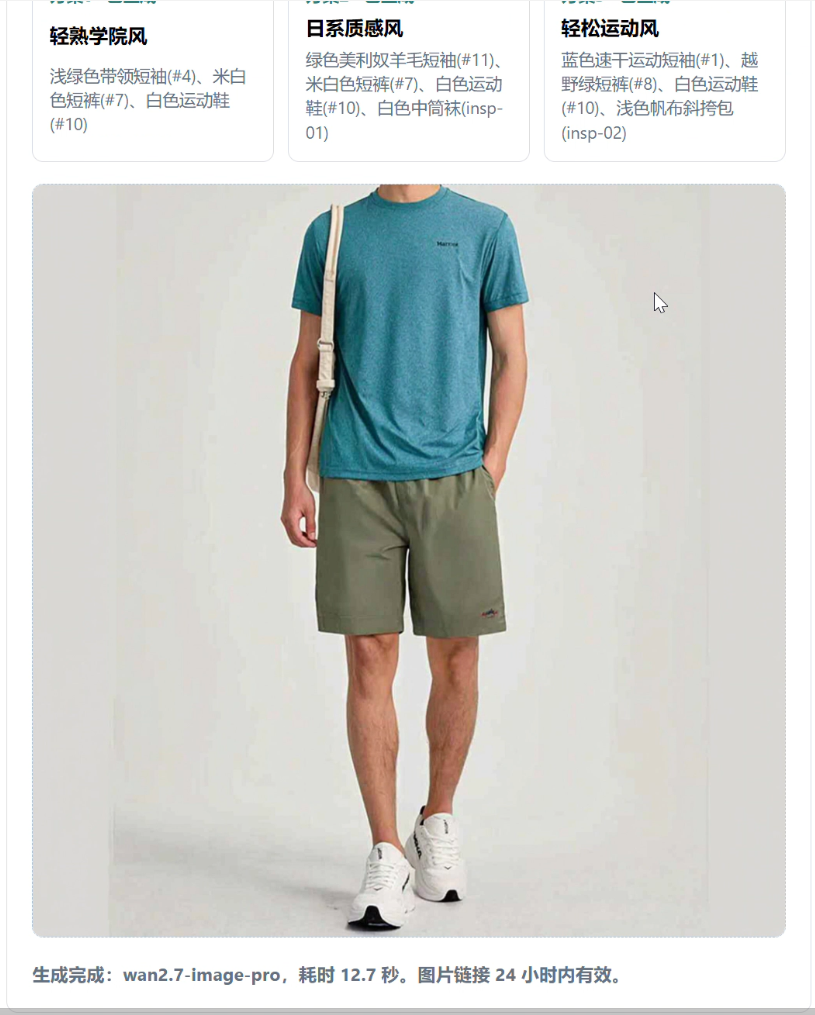
\includegraphics[width=\linewidth]{figures/match3.png}
        \caption{生成的方案三的穿搭效果参考图。}
        \label{fig:match3}
    \end{minipage}

\end{figure}

在这里值得讨论的是，我们搭建项目时，对于虚拟上身效果图生成 Prompt 的添加与不断调整耗费了许多时间。
在初始阶段，我们的 Prompt 只要求大模型根据给定的穿搭方案、用户衣柜和灵感衣物文字输出一张可供用户参考穿搭的效果图，
模型就表现得相当不错 ———— 它仿佛知道我们想要的参考图样式，我们尝试了许多轮，它都生成了符合要求的图片；
但当\textbf{帽子}这个元素加入穿搭后，事情便开始变得复杂了起来。
我们发现它在生成含有帽子元素的参考图时，生成的图片会含有面部信息，当然在这种情境下这是可接受的；
不可接受的是，我们随后又让它生成一些穿搭中不含有帽子元素的参考图，但它似乎着迷于在图中生成人脸，
生成的几张图片中又都包含面部信息。
于是，我们对后端的 Prompt 进行了一轮调整，让模型在穿搭中不含帽子、丝巾等头饰元素时生成从脖子处裁切的穿搭参考图，
有头饰元素时则生成全身穿搭效果参考图。
调整后的 Prompt 的确带来了一些优化，在穿搭不含头饰时模型不再会生成含有面部信息的参考图；
然而，我们很快又发现，模型总是会生成从腰部裁剪的参考图，上半身穿搭效果不直观。
因此，我们又对 Prompt 进行了几轮添加调整，多次强调模型生成参考图的裁剪位置。
但过分的语言强调反而带来了反作用，模型生成参考图的质量相比之前不增反降。
由此我们开始思考 Prompt 长度的问题，过长的 Prompt 可能让模型难以抓住核心，
从而使它抛弃其中的一些生成要点而紧抓看似重要实则影响轻微的东西。
所以，经过又几轮不断调整尝试，我们最终删去了原本的许多反复限制约束，明确了 Prompt 生成合适尺度参考图的核心：
\textbf{如果方案中没有帽子元素，则要求必须生成从脖子到鞋子的全身人像，完整露出肩线的同时避免生成用户本人或露脸图；
如果方案中有帽子，则允许完整展示头部和帽子。}
调整后，模型生成参考图的质量明显提升了许多，也不再频繁生成面部信息，或是在腰部裁剪图片。

在运用万相模型生成参考图的同时，
我们还运用了 OpenAI 公司的 GPT-Image-2 模型生成相同 Prompt 的参考图作为实验对比。
我们发现，输入同样的、清晰明确程度均一致的 Prompt ，Image-2 相比万相更能捕捉到其中的要点，
很少出现生成不符合要求参考图的情况，并且生成图像的模特、穿搭质感相比万相来的更加真实。
这种对比也让我们切身地意识到，技术上国产大模型相较于国际先进模型仍有较大提升空间。
但从 token 的使用成本上而言，国产大模型具有很强优势，因此我们综合考虑后在项目中运用了千问万相文生图模型。

\subsection{实验小结}

上述全流程实验可以看出，我们搭建的 AIWardrobe 助手能够完成从用户输入到最终穿搭可视化的完整流程。
需求解析模块将自然语言输入转化为结构化输入， RAG 检索模块提供真实穿搭案例作为参考，
穿搭生成模块在衣柜约束下给出三套可执行方案，前端证据区和校验区提高方案可解释性，
虚拟上身模块则进一步降低了用户理解穿搭效果的思考成本。

与此同时，实验也暴露出我们项目的一些不足。
首先，我们构建起的 RAG 样例库规模仍然较小，且主要依赖人工整理的文本描述，覆盖的风格和场景有限；
其次，图像生成的穿搭参考图虽然具有参考价值，但仍可能出现局部细节与真实衣物不完全一致的问题；
最后，当前对穿搭的评价方式主要基于案例观察和人工判断，
后续可以结合时尚设计领域的相关知识设计更系统的用户评分实验，
从满意度、可穿性、风格匹配度和衣柜利用率等维度更加量化评估助手表现。




\addcontentsline{toc}{section}{参考文献}
\bibliographystyle{ieeetr}
\bibliography{ref}


\end{document}
